\documentclass[letter]{article}
\usepackage[utf8]{inputenc}
\usepackage[margin=1in]{geometry}
\usepackage{tikz}
\usepackage{ulem}
\usepackage{graphics}
\usepackage{sidecap}
\usepackage{wrapfig}
\usepackage[toc,page]{appendix}
\usepackage{caption}
\usepackage{amssymb}
\usepackage{amsmath}
\usepackage{algorithmicx}
\usepackage{algpseudocode}

\usepackage{url,graphicx,tabularx,array,geometry,amsmath,tikz}
\usepackage{algorithm}% http://ctan.org/pkg/algorithms
\usepackage{algpseudocode}% http://ctan.org/pkg/algorithmicx
\usepackage{listings}
\usetikzlibrary{arrows}
\newenvironment{myindentpar}[1]% %indent whole paragraph when needed
 {\begin{list}{}%
         {\setlength{\leftmargin}{#1}}%
         \item[]%
 }
 {\end{list}}

\usepackage{hyperref}
\usepackage{parskip}

\lstset{
  basicstyle=\small,
  stringstyle=\ttfamily,
  numbers=left,
  numberstyle=\tiny,
  stepnumber=1, 
  numbersep=5pt,
  language=R }

\hypersetup{
    colorlinks,%
    citecolor=black,%
    filecolor=black,%
    linkcolor=black,%
    urlcolor=black
}

\def\dashuline{\bgroup 
  \ifdim\ULdepth=\maxdimen  % Set depth based on font, if not set already
	  \settodepth\ULdepth{(j}\advance\ULdepth.4pt\fi
  \markoverwith{\kern.15em
	\vtop{\kern\ULdepth \hrule width .3em}%
	\kern.15em}\ULon}
\setlength\parindent{2em}

\newcounter{foot}
\setcounter{foot}{1}

\author{Olga Prilepova, Christopher Patton, Alexander Rumbaugh, \\ John Chen, Thomas Provan}

\date{\today}
\title{ECS256 - Final project}
	
\begin{document}
\maketitle


%%%%%%%%%%%%%%%%%%%%%%%%%%%%%%%%%%%%%%%%%%%%%%%%%%%%%%%%
\section*{Problem 1} 

As suggested by the hint, in order to find the bias at $t=0.5$, we're going to be examining the value of $\beta$ as n goes to $\infty$. The idea behind this is that the proposed model will converge to some $\beta$ as the number of samples increases, to the point that it fits as closely as possible to the actual function. Of course, it isn't possible for the model to fit precisely, because the actual relationship isn't linear like the model is, so there will be some bias in the resulting model. 

The first thing to consider is model construction. The simplest way to construct the model would be to use a least-squares method, so in the construction we would  minimize the following with respect to $g(X)$, which is the set of all possible functions for our model.

\begin{equation}
	E[(EY - g(X))^2]
\end{equation}

For this problem, $g(X)=\beta X$ for all possible $\beta$, and the actual distribution of $EY$ is $X^{0.75}$, so we can rewrite this to minimizing the following with respect to $\beta$

\begin{equation}
	E[(X^{0.75} - \beta X)^2]
\end{equation}

To actually find this value, we will first make a new variable $Q=(X^{0.75} - \beta X)^2$, and then use the continuous case of iterated expectations along X (eq 5.33) to find $EQ$

\begin{equation}
	EQ = \int _{-\infty} ^\infty f_X(t) \; E(Q | X = t)\; dt
\end{equation}

\begin{equation}
	E(Q | X = t) = E[(t^{0.75} - \beta t)^2] = (t^{0.75} - \beta t)^2
\end{equation}

X is $U(0,1)$, so $f_X(t)$ is 1 between the values of 0 and 1, and is zero elsewhere. With this and the value of $E(Q | X = t)$, we can rewrite $EQ$ as the following.

\begin{equation}
	EQ = \int _0 ^1 (t^{0.75} - \beta t)^2 \; dt
\end{equation}

From here it's a simple matter to minimize with respect to $\beta$. First, finish computing the integral to get the final function of $\beta$ to minimize.

\begin{equation}
	EQ = \frac{1}{3}(\beta^2 - \frac{24}{11}\beta + \frac{6}{5})
\end{equation}

And then take the derivative of the function with respect to $\beta$.

\begin{equation}
	\frac{d\,EQ}{d\beta} = \frac{2}{3}\beta - \frac{8}{11}
\end{equation}

And finally set that equal to zero and solve for $\beta$, which yields $\beta=\frac{12}{11}$ as the value that minimizes our function.

Now we can move on and compute the bias. The bias is simply $\hat{m}_{Y;X}(t) - m_{Y;X}(t)$, which for the selected $\beta$ and $t=0.5$ is

\begin{equation}
	Bias(0.5) = \beta 0.5 - 0.5^{0.75} \approx {\fbox {\parbox{0.5in}{-0.0491}}}
\end{equation}

%%%%%%%%%%%%%%%%%%%%%%%%%%%%%%%%%%%%%%%%%%%%%%%%%%%%

\section*{Problem 2.a}

For convenience, we give the call forms of the important routines:
\begin{itemize}
  \item \texttt{prsm(y,x,k=0.01,predacc=ar2,crit="max",printdel=F)} 
  \item prediction accuracy criteria: \texttt{ar2(y, x)}, \texttt{aiclogit(y, x)}
\end{itemize}

Our implementation of \texttt{prsm()}\footnote{See \texttt{Parsimony.R} in the project folder.} 
honors the program's specification. We first calculated the PAC ("prediction accuracy criterion")
with all predictor variables. Next, we removed the first attribute from the predictor variables 
and recalculated the PAC with the new parsimony. If the PAC has improved, or has only degraded 
marginally, we accept it as our new target PAC and the set of attributes as our new parsimony.
We repeat this procedure for the next attribute, using the modified parsmony. This process is 
repeated for all attributes. For continuous regression, we used the adjusted $R^2$ for the PAC; 
for logstic regression, we used the AIC.

One of our goals in this project was to validate this greedy approach to reducing parsimony. 
Let $\text{PAC}^*$ be our target prediction accuracy criterion. Using AIC in logistic regression,
the goal of \texttt{prsm()} is to find a smallest subset of the predictor variables with minimal
PAC value, but no greater than $(1+k)\cdot\text{PAC}^*$. (The goal is analogous for continuous regession 
with adjusted $R^2$, except we maximize this value.) 

It's easy to see that \texttt{prsm()} will not find
the optimal parsimony in general. Suppose we start with predictor variables 
$\{X^{(1)}, X^{(2)}, X^{(3)}, X^{(4)}, X^{(5)}\}$ 
and response variable $Y$. Suppose at some point we remove $X^{(2)}$ from the parsimony,
since $\texttt{aiclogit}(Y, \{X^{(1)}, X^{(3)}, X^{(4)}, X^{(5)}\}) < (1+k)\cdot\text{PAC}^*$.  
If the optimal parsiomny includes $X^{(2)}$, but excludes variables we would delete later on, 
then we won't ever reach it. We affectively cut off a branch of computation that would have 
lead to a better, if not globablly optimal solution. Intuitively, we see that the order in 
which the attributes are successively removed determines the resulting PAC value and 
parsimony.

To address this apparent problem, we implemented an exhaustive search version, called 
\texttt{prsmpwr()}, which minimizes the PAC (or maximizes in the case of continuous 
regression) over all subsets of the attributes. We iterate over the power set of the 
predictor variables from smallest to largest. We accept the new parsimony if the PAC
is less than $(1+k)\cdot\text{PAC}^*$; however, we only accept a new $\text{PAC}^*$  
if it is strictly less than the old target.











%\lstinputlisting{figures/prsm_fig.R}


\subsection*{Problem 2.b}

First, the results requested from the simulated data in tabular form. The variables listed in the table are the variables that were selected by the specified method for each run.


\begin{tabular}{| l  r | c | c | c |}

\hline

	&&	prsm(k=0.01)&	prsm(k=0.05)&	sig test	\\
\hline

n=100&	Run 1&	$X_1 ,X_2, X_3, X_9$&	$X_1, X_2, X_3$&		$X_1, X_2, X_3$	\\
	&	Run 2&	$X_1, X_2, X_3$&		$X_1, X_2, X_3$&		$X_1, X_2, X_3$	\\
	&	Run 3&	$X_1, X_2, X_3$&		$X_1, X_2, X_3$&		$X_1, X_2, X_3$	\\

\hline

n=1000&	Run 1&	$X_1, X_2, X_3$&		$X_1, X_2, X_3$&		$X_1, X_2, X_3, X_4$	\\
	&	Run 2&	$X_1, X_2, X_3$&		$X_1, X_2, X_3$&		$X_1, X_2, X_3$		\\
	&	Run 3&	$X_1, X_2, X_3$&		$X_1, X_2, X_3$&		$X_1, X_2, X_3$		\\
	
\hline
			
n=10000&	Run 1&	$X_1, X_2, X_3$&		$X_1, X_2, X_3$&		$X_1, X_2, X_3, X_4$		\\
	&	Run 2&	$X_1, X_2, X_3$&		$X_1, X_2, X_3$&		$X_1, X_2, X_3, X_4$		\\
	&	Run 3&	$X_1, X_2, X_3$&		$X_1, X_2, X_3$&		$X_1, X_2, X_3, X_4, X_9$		\\

\hline
			
n=100000&	Run 1&	$X_1, X_2, X_3$&		$X_1, X_2, X_3$&		$X_1, X_2, X_3, X_4$		\\
	&	Run 2&	$X_1, X_2, X_3$&		$X_1, X_2, X_3$&		$X_1, X_2, X_3, X_4, X_9$		\\
	&	Run 3&	$X_1, X_2, X_3$&		$X_1, X_2, X_3$&		$X_1, X_2, X_3, X_4, X_9$		\\

\hline

\end{tabular}


As the table shows, each method consistently keeps the most important 3 $X_i$'s in all of our test runs. The smaller k value seems to be less willing to discard variables at low n values, indicated by it selecting the irrelevant X9 variable, but at higher n values it seems to consistently discard the unimportant variables. The sig test, on the other hand, appears to become more willing to accept irrelevant X's as we increase n. However, it is also worth noting that it starts consistently picking out the relevant, but weakly influencing variable X4, which the parsimony methods seems to always discard at high values of n, and rarely pick up at low values.

However, this analysis felt insufficient to us. Three runs isn't nearly enough to see any patterns, and some results may be pure chance! For example, notice how the only completely irrelevant value it chose was $X_9$. Each of these trials were independent from each other, so the methods should have been no more likely to select $X_9$ from any of the five irrelevant variables. This indicated to us that this is not enough trials to show us anything about the data. To investigate further, we ran each analysis method 100 times on distinct samples of our data, and then compiled the following tables. The value in the table is the proportion of our 100 trials that each method selected the particular variable $X_i$.

\begin{tabular}{| l | c | c | c | c | c | c | c | c | c | c |}



\hline
\textbf{prsm(k=0.01)}&	$X_1$&	$X_2$&	$X_3$&	$X_4$&	$X_5$&	$X_6$&	$X_7$&	$X_8$&	$X_9$&	$X_{10}$\\
\hline
N = 100&			1&	1&	1&	0.24&	0.11&	0.14&	0.21&	0.22&	0.26&	0.28 	\\
N = 1000&			1&	1&	1&	0.08&	0&	0&	0&	0&	0&	0	\\
N = 10000&			1&	1&	1&	0&	0&	0&	0&	0&	0&	0	\\
N = 100000&		1&	1&	1&	0&	0&	0&	0&	0&	0&	0	\\
N = 1M&			1&	1&	1&	0&	0&	0&	0&	0&	0&	0	\\
\hline		

\\
								
									\\		
\hline					
\textbf{prsm(k=0.05)}&	$X_1$&	$X_2$&	$X_3$&	$X_4$&	$X_5$&	$X_6$&	$X_7$&	$X_8$&	$X_9$&	$X_{10}$\\
\hline
N = 100&			1&	1&	0.99&	0.1&	0.02&	0.05&	0.04&	0.03&	0.07&	0.02	\\
N = 1000&			1&	1&	1&	0&	0&	0&	0&	0&	0&	0	\\
N = 10000&			1&	1&	1&	0&	0&	0&	0&	0&	0&	0	\\
N = 100000&		1&	1&	1&	0&	0&	0&	0&	0&	0&	0	\\
N = 1M&			1&	1&	1&	0&	0&	0&	0&	0&	0&	0	\\
\hline
\\

								
											\\
\hline
\textbf{Sig Test}&	$X_1$&	$X_2$&	$X_3$&	$X_4$&	$X_5$&	$X_6$&	$X_7$&	$X_8$&	$X_9$&	$X_{10}$\\
\hline
N = 100&		1&	1&	1&	0.14&	0.03&	0.05&	0.05&	0.03&	0.09&	0.04	\\
N = 1000&		1&	1&	1&	0.31&	0.02&	0.05&	0.05&	0.05&	0.02&	0.04	\\
N = 10000&		1&	1&	1&	1&	0.04&	0.01&	0.07&	0.07&	0.03&	0.06	\\
N = 100000&	1&	1&	1&	1&	0.35&	0.06&	0.09&	0.03&	0.05&	0.03	\\
N = 1M&		1&	1&	1&	1&	1&	0.05&	0.03&	0.08&	0.02&	0.03	\\
\hline
\end{tabular}

This gives us a much more complete picture of the situation. As we suggested earlier, it appears that all of the methods very easily find that $X_1$, $X_2$, and $X_3$ are important to the model, and select them in every simulated data set. (with one exception) This is still an uninteresting conclusion, but now it's much more solidly demonstrated than from just three dataruns. More interesting is the behavior of the other columns, which we previously could not say much about, since we only had the three simulations.

First, we will examine the behavior of methods on the two weakly influencing variables, $X_4$ and $X_5$. The \textbf{prsm} methods seem to be more likely to pick up on these weakly influencing variables at low $n$ values, but discard them completely at higher $n$ values. Additionally, it seems as if setting lower tolerance values increases \textbf{prsm}'s ability to pick up on these weakly influencing values. However, this only seems to take place at reasonable $n$. At $n=100$, \textbf{prsm} seems to lose the weakly influencing variables regardless of k value. We did test $k=0.005$ briefly to explore this. At $n=100$, \textbf{prsm} didn't select the weak values any more often than the irrelevant variables, but at $n=1000$ it selected the weak variable $X_4$ significantly more often than the irrelevant variables. As with other $k$ values, however, this proportion dropped as $n$ increased. The significance test, on the otherhand, started to pick up the weakly influencing variables as $n$ increased. For the highest $n$, the significance test always selected the weakly relevant variables. 

Now we will look at the second group, the irrelevant variables. \textbf{prsm} very quickly discarded all of the irrelevant variables as $n$ increased. For both $k$ values we looked at (and the smaller $k$ we examined briefly), \textbf{prsm} selected none of the irrelevant variables by $n=1000$. Significance testing, however, never fully stopped selecting irrelevant variables. Even at our highest $n$, the significance test still selected irrelevant variables as part of the predictor, and with roughly the same probability as it had at lower $n$. Increasing $n$ seems to have no impact on significance test's likelyhood to select one of the irrelevant variables.

Between the two, this allows us to draw some interesting contrast between the two models. The \textbf{prsm} models very quickly zero in on the most critical variables for creating it's estimate and remove irrelevant variables with a comparatively low sample size, but can lose subtle variables with small impacts on the distribution. In contrast, significance testing will consistently find relevant variables, getting better at finding and including subtle effects as $n$ increases, but at the cost of being unable to fully exclude irrelevant variables at any point.

Perhaps this suggests another model, where we use these two models to cover each others weaknesses. \textbf{prsm} is very good at finding the most relelvant variables, and seems to be able to easily point out the most important variables for a model to consider. But if we need to consider finer aspects, perhaps we could use the Sig Test method (or something similar and a little more sophisticates) to aid in finding subtle variables to add to the \textbf{prsm}'s list.



\section*{Problem 2.c}

\subsection*{Abalone, ~\cite{abalone} (continuous and logistic, small $p$, small $n$)}

The Abalone data set is fairly small in the number of observations and dimensions. The only variable that wasn't numeric was Sex. We changed the nominal Sex variable from F,M,I (Male, Female or Infant) into is.male and is.infant (each 0-1 valued). For logistic regression we used is.infant variable as the response variable.

\begin{center}
    \begin{tabular}{ | l |  p{4cm} |  p{4cm} | p{4cm} |}
    \hline
    Method & Parsimony (k = 0.01) & Parsimony (k = 0.05) & Significance Testing \\ \hline
    	
    Columns Retained & is.male, length, viscerra.weight, rings & is.male, shell.weight & length, diameter, whole.weight, viscerra.weight, rings\\ \hline
    
    AIC & 2150.704 & 2303.834 & 3318.3\\ \hline
    
    \end{tabular}
\end{center}

The AIC reported after using our parsimony function is lower for k=0.01, and the number of explanatory variables remaining is smaller than the number of significant explanatory variables according to significance testing performed. This is one of those cases where parsimony function works better than significance testing in identifying a smaller subset of important explanatory variables.

Shell Weight was chosen as the response variable for continuous case analysis.

\begin{center}
    \begin{tabular}{ | l |  p{4cm} |  p{4cm} | p{4cm} |}
    \hline
    Method & Parsimony (k = 0.01) & Parsimony (k = 0.05) & Significance Testing \\ \hline
    	
    Columns Retained & whole.weight, shucked.weight & whole.weight & diameter, height, whole.weight, shucked.weight, viscerra.weight, rings\\ \hline
    
    Adjusted RSquared & 0.9440963 & 0.9126831 & 0.953487\\ \hline
    
    \end{tabular}
\end{center}

Our parsimony function performs almost as well as the significance testing approach and it is using only 2 explanatory variables. It works very well for this small and very straightforward data set.

\subsection*{Median House Values \cite{cadata} (continuous, small $p$, large $n$)}
Our next data set explores house value throughout California derived from 1990 census data. The state is divided up into 20640 geographic blocks with average population 1425.

We are interested in how the following variables affect median house value: median income, housing median age, total rooms, total bedrooms, population, households, latitude, and longitude.

Here is R's summary output of the data:
\begin{verbatim}
Median.House.Value Median.Income       Median.Age   
 Min.   : 14999     Min.   : 0.4999   Min.   : 1.00  
 1st Qu.:119600     1st Qu.: 2.5634   1st Qu.:18.00  
 Median :179700     Median : 3.5348   Median :29.00  
 Mean   :206856     Mean   : 3.8707   Mean   :28.64  
 3rd Qu.:264725     3rd Qu.: 4.7432   3rd Qu.:37.00  
 Max.   :500001     Max.   :15.0001   Max.   :52.00
Total.Rooms    Total.Bedrooms     Population   
 Min.   :    2   Min.   :   1.0   Min.   :    3  
 1st Qu.: 1448   1st Qu.: 295.0   1st Qu.:  787  
 Median : 2127   Median : 435.0   Median : 1166  
 Mean   : 2636   Mean   : 537.9   Mean   : 1425  
 3rd Qu.: 3148   3rd Qu.: 647.0   3rd Qu.: 1725  
 Max.   :39320   Max.   :6445.0   Max.   :35682
 Households        Latitude       Longitude     
 Min.   :   1.0   Min.   :32.54   Min.   :-124.3  
 1st Qu.: 280.0   1st Qu.:33.93   1st Qu.:-121.8  
 Median : 409.0   Median :34.26   Median :-118.5  
 Mean   : 499.5   Mean   :35.63   Mean   :-119.6  
 3rd Qu.: 605.0   3rd Qu.:37.71   3rd Qu.:-118.0  
 Max.   :6082.0   Max.   :41.95   Max.   :-114.3  
 \end{verbatim}

 
 Next we use our Parsimony package on the data at various k levels. Here are the calls and output:
\begin{verbatim}
 > prsm(df[,1],df[,2:9],k=0.01, predacc=ar2, crit='max', printdel=T)
full outcome =  0.6369649 
deleted         Total.Rooms 
new outcome  =  0.6350863 
deleted         Total.Bedrooms 
new outcome  =  0.6321316 
[1] "Median.Income" "Median.Age"    "Population"    "Households"    "Latitude"      "Longitude"
\end{verbatim}
\begin{verbatim}
> prsm(df[,1],df[,2:9],k=0.05, predacc=ar2, crit='max', printdel=T)
full outcome =  0.6369649 
deleted         Median.Age 
new outcome  =  0.6243571 
deleted         Total.Rooms 
new outcome  =  0.6218261 
deleted         Total.Bedrooms 
new outcome  =  0.6198323 
[1] "Median.Income" "Population"    "Households"    "Latitude"      "Longitude"
 \end{verbatim}
By loosening our k value, the model selector decides to remove Median Age in the latter run. It is interesting to note that longitude and latitude remain in the model, which we will address later.

Next we want to compare our Parsimony package to the significance testing approach. 

Here is the summary of the coefficients of our lm() call in R:
\begin{verbatim}
Coefficients:
                 Estimate Std. Error t value Pr(>|t|)    
(Intercept)    -3.594e+06  6.254e+04 -57.468  < 2e-16 ***
Median.Income   4.025e+04  3.351e+02 120.123  < 2e-16 ***
Median.Age      1.156e+03  4.317e+01  26.787  < 2e-16 ***
Total.Rooms    -8.182e+00  7.881e-01 -10.381  < 2e-16 ***
Total.Bedrooms  1.134e+02  6.902e+00  16.432  < 2e-16 ***
Population     -3.854e+01  1.079e+00 -35.716  < 2e-16 ***
Households      4.831e+01  7.515e+00   6.429 1.32e-10 ***
Latitude       -4.258e+04  6.733e+02 -63.240  < 2e-16 ***
Longitude      -4.282e+04  7.130e+02 -60.061  < 2e-16 ***
--- 
\end{verbatim}
The significance testing approach deletes no predictors. This data set has a large size (20640) so it makes sense that the predictors are all deemed significant.

Here is a summary of the comparison of methods:

\begin{tabular}{ | c | p{3cm} | p{3cm} | c  |}
\hline
Method&Parsimony (k=0.01) & Parsimony (k=0.05) & Significance Testing \\
\hline
Columns\newline Deleted& Total Rooms \newline Total Bedrooms & Total Rooms \newline Total Bedrooms \newline Median Age & None \\
\hline
Adjusted RSquared & 0.6321316 & 0.6218261 & 0.6369649 \\
\hline
\end{tabular}

Before discussing conclusions about the data, we address latitude and longitude. Looking at the full summary above, latitude and longitude both have negative coefficient values. This says if we travel east or north, on average house value decreases. However a real estate expert would think you are crazy hearing that statement.

The problem arises with using coordinate data in a linear regression model. Without any interaction terms we are assuming the statement above. We would risk overfitting if we attempted to make a complex formula involving coordinates. 

A block's location is clearly important. We can see what blocks are close to one another, and proximity to oceans or mountains. Using location data effectively can lead to powerful models, however our model is not set up to do this. But we can plot our data atop a map which we will show shortly.

We remove latitude and longitude and use the predictors kept by our Parsimony package. Here is the summary of the regression:
\begin{verbatim}
Coefficients:
                Estimate Std. Error t value Pr(>|t|)    
(Intercept)   -32165.268   2167.358  -14.84   <2e-16 ***
Median.Income  43094.918    284.263  151.60   <2e-16 ***
Median.Age      2000.544     45.080   44.38   <2e-16 ***
Population       -43.045      1.127  -38.20   <2e-16 ***
Households       152.700      3.344   45.66   <2e-16 ***
\end{verbatim}
First we see that income positively affects house value which is unsurprising. If people have more income, they can afford more expensive houses.

Next looking at age, we see it also positively affects house value. One would expect older people to have more money and this reflected in the high co-variance between these predictors.

Moving onto population, we see it negatively affects house value. With this data set each block has approximately similar geographic size, so blocks with higher population can be assumed to be denser. From our model we can conclude less dense areas have higher housing value. 

Finally we look at number of households which positively affects house value. This is a bit surprising since population had a negative coefficient. One possible explanation is that our model is detecting large suburban areas which are all houses. Areas with more apartment complexes would fewer number of households and also lower housing value.

Parsimony simplified our model down to four predictors. While we lost the data about rooms, we still have a model we can clearly understand.  

Now we make use of our coordinate data using R's ggmap library. First we looked at a map of California as a whole, then zoomed into the Bay Area and the Greater Los Angeles area.

\newpage
\begin{figure}[H]
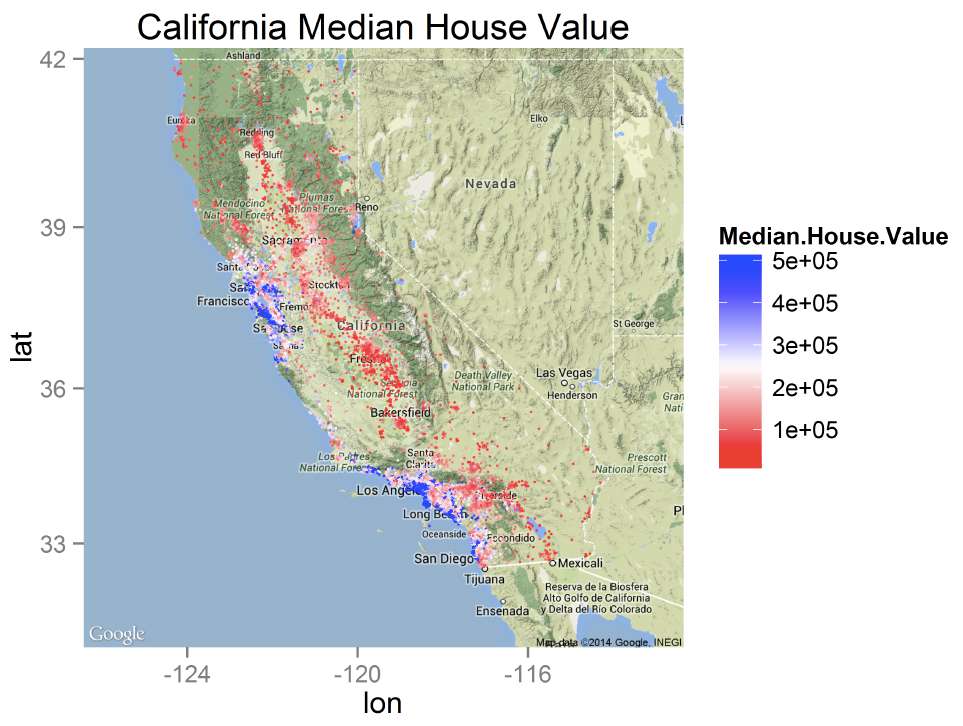
\includegraphics[scale=.25]{figures/california.png}
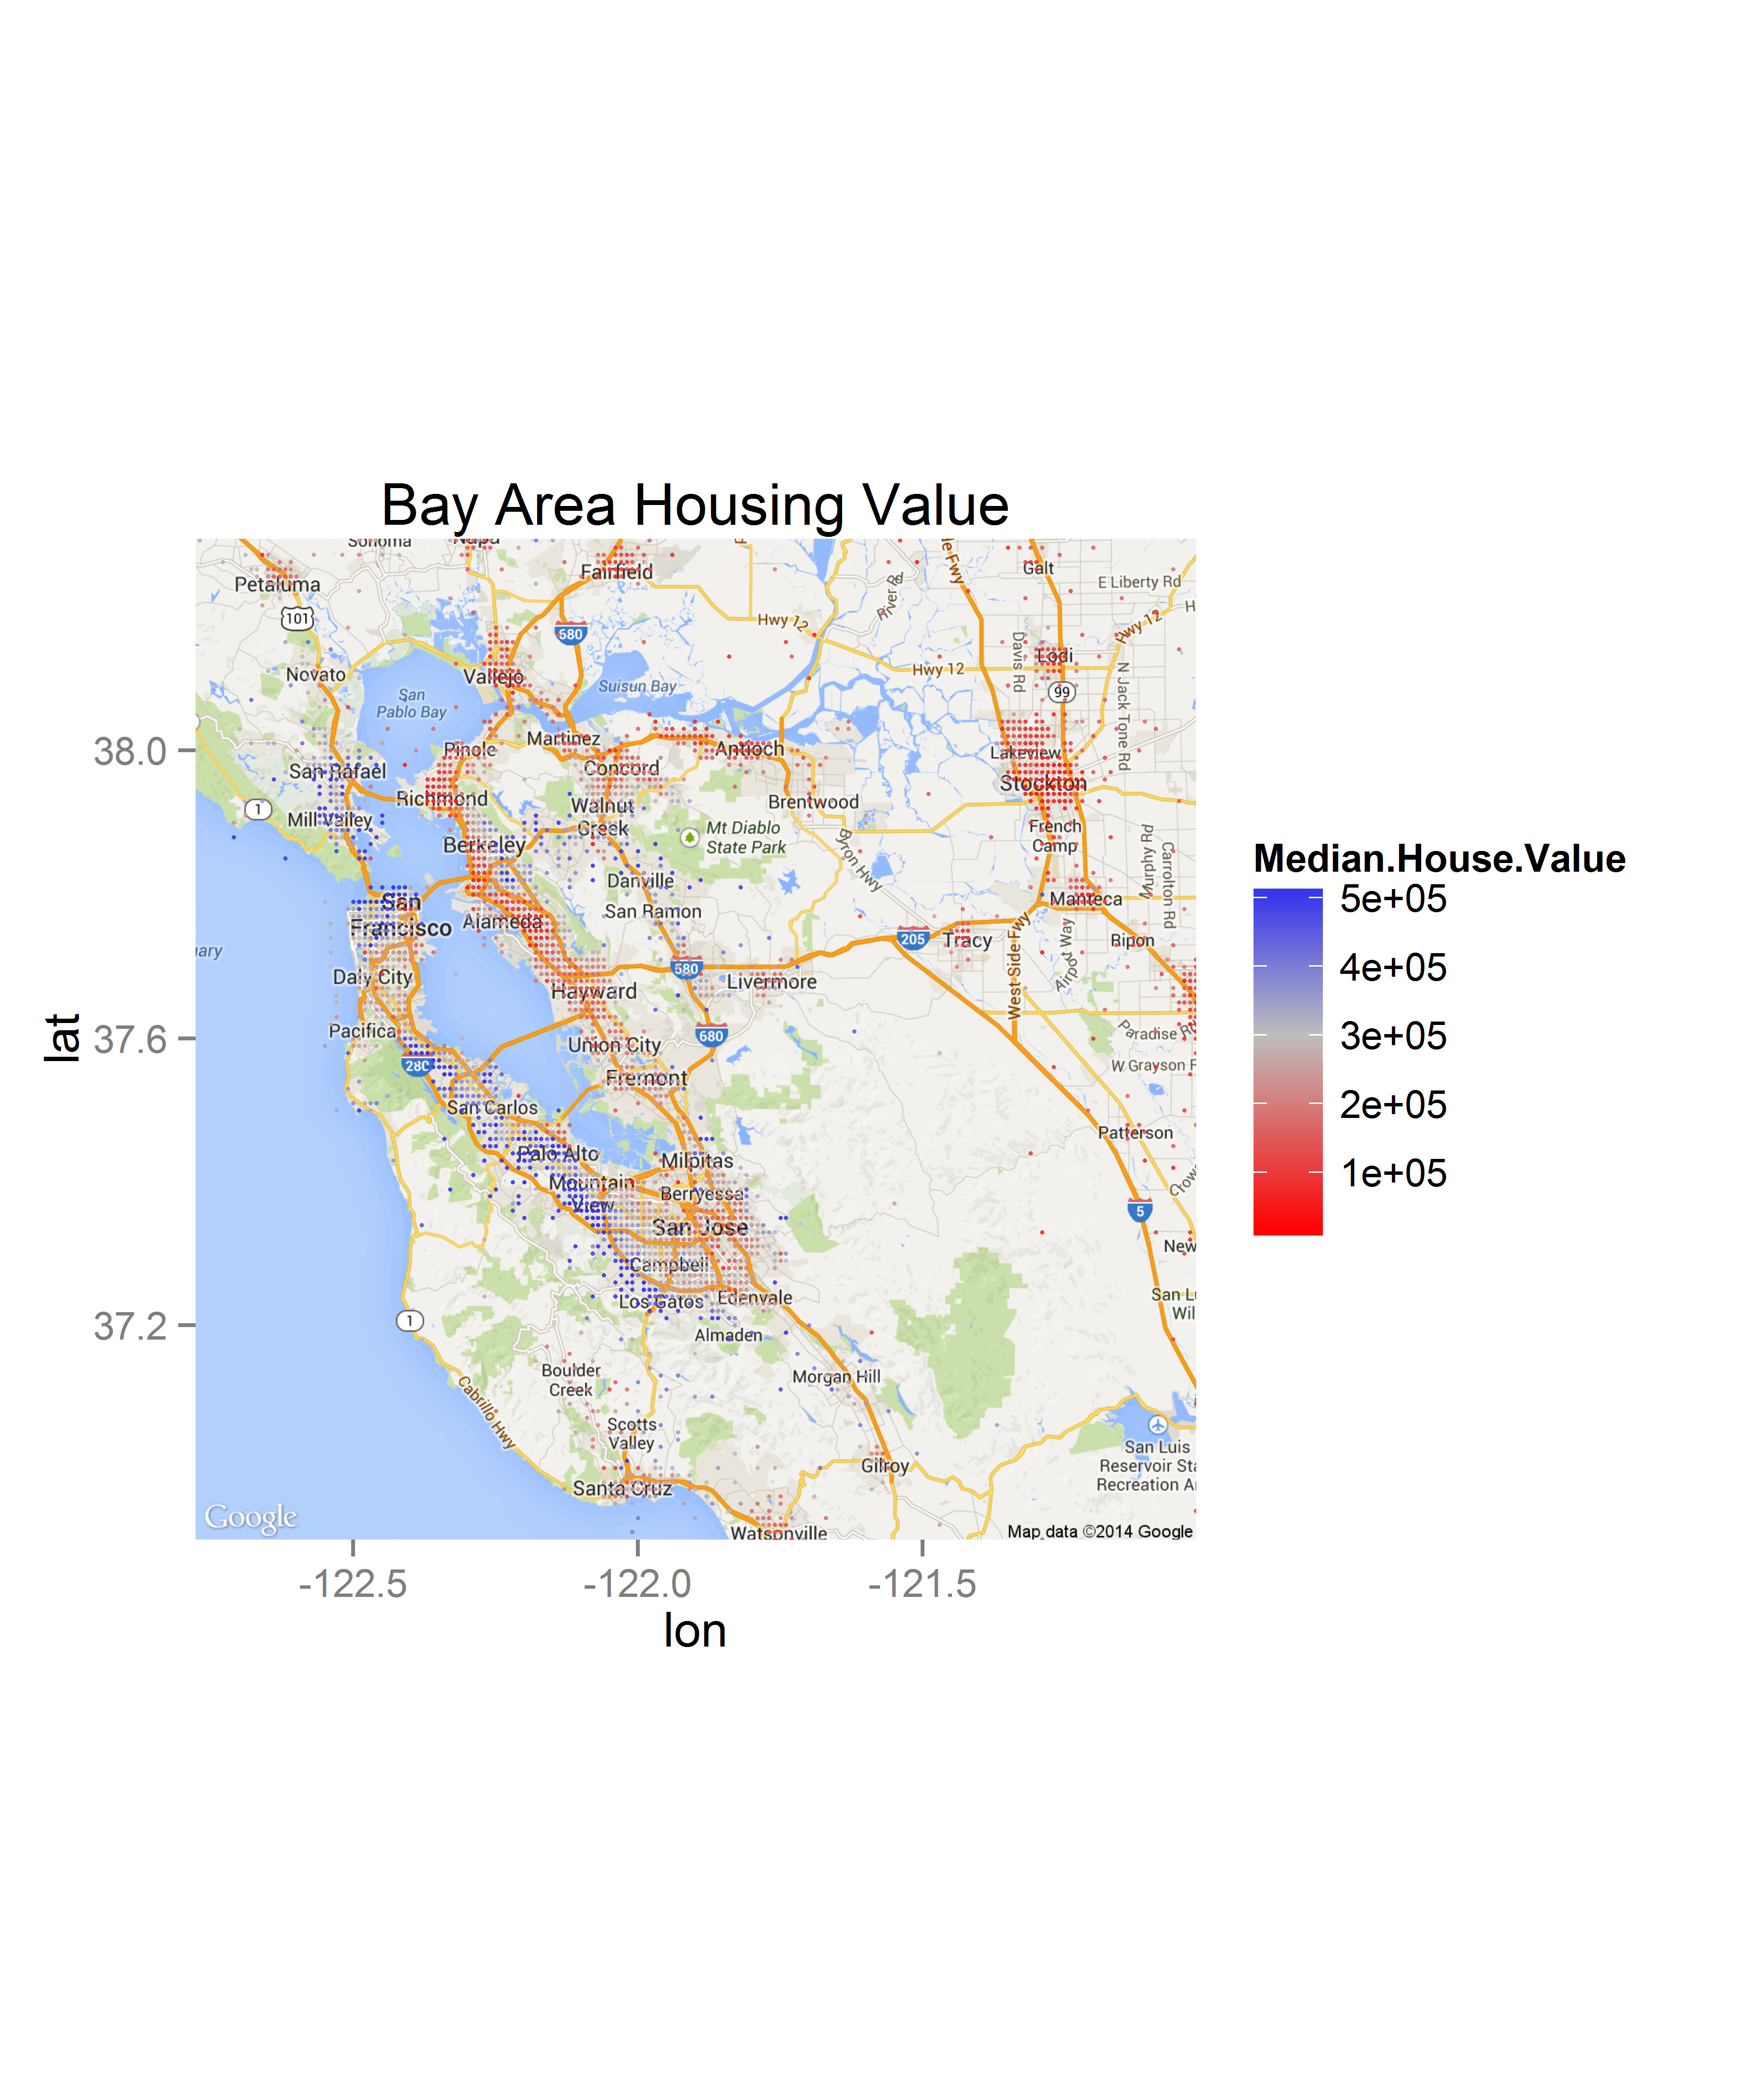
\includegraphics[scale=.25]{figures/bayarea.png}
\includegraphics[scale=.5]{figures/losangeles.png}
\end{figure}

The visualization helps us see how housing value is clustered in the state. As one might expect, rural areas generally have lower housing value than metropolitan areas. Within the metropolitan areas there are visible divisions as well. 




\subsection*{Space Shuttle \cite{shuttle} (logistic, small $p$, large $n$)}
Next we looked at space shuttle data taken from the UCI Machine Learning Repository. The goal was to predict the class given 8 predictors, with 43500 data points. Our logistic regression predicted whether or not the class was of type 1.  The description of the data set was very poor, however it matched our criterion for dimension, data points, and regression type. Because of the lack of sufficient description, few conclusions can be drawn from the data, but we can still test our Parsimony package.

Here is the summary of results using Parsimony:

\begin{tabular}{ | c | p{3cm} | p{3.3cm} | c  |}
\hline
Method&Parsimony (k=0.01) & Parsimony (k=0.05) & Significance Testing \\
\hline
Columns Deleted& V1,V3,V4,V6,V9 & V1,V2,V3,V4,V6,V9 & V4 \\
\hline
AIC & 8575.803 & 8728.906 & 8475.2 \\
\hline
\end{tabular}

We also tested the various methods against a validation training set. We looked at the probability of correctly identifying a class 1 or not class 1. Also if we identified something as class 1, what was the probability it was actually class 1 and the same for not class 1.

Here is a summary of the results:

\begin{tabular}{ | c | p{3cm} | p{3.3cm} | c  |}
\hline
Method&Parsimony (k=0.01) & Parsimony (k=0.05) & Significance Testing \\
\hline
P(Correct ID $|$ class 1) & 0.9862345 & 0.9861474 & 0.9864959 \\
\hline
P(Correct ID $|$ not class 1) & 0.9285242 & 0.9285242 & 0.9169424 \\
\hline
P(Correct ID $|$ guess class 1) & 0.981276 & 0.9812744 & 0.9783135 \\
\hline
P(Correct ID $|$ guess not class 1) & 0.9466937 & 0.9463744 & 0.9470267  \\
\hline
\end{tabular}

The results for the different methods are very close and it is hard to detect much difference in the accuracy levels. There were slightly fewer false positives and there was a slightly better detection of negatives for the Parsimony models. By simplifying the model, there is a possibility of increased accuracy during validation runs.
\\
\\


\subsection*{Census, 1994~\cite{census} (continuous and logistic, large $p$, large $n$)}
Here we are analyzing Census data which contains 32561 observations, 13 variable vectors and is based on the 1994 Census. There are several categorical variables in this data set. In order to accommodate regression modeling each categorical vector was split into 0-1 valued vectors for each category. According to the website from which the data set was taken the goal was to predict whether a given person would be making over 50K a year.  Our parsimony function at k=0.1 eliminated all but one explanatory variable, which turned out to be "capital gain". 
\begin{verbatim}
Coefficients:
              Estimate Std. Error t value Pr(>|t|)    
(Intercept)  2.269e-01  2.334e-03   97.19   <2e-16 ***
capital.gain 1.293e-05  3.128e-07   41.34   <2e-16 ***
---

\end{verbatim}

This makes sense. If we were to look at only one column in order to predict if a person is making over 50K a year, the capital gain variable would be most informative. At k=0.01 there are many more explanatory variables that enhance the predictions:  "age", "education.num", "Exec.managerial", "Not.in.family", "Own.child", "Unmarried", "Wife", "capital.gain", "capital.loss", "hours.per.week".

\begin{verbatim}
Coefficients:
                  Estimate Std. Error t value Pr(>|t|)    
(Intercept)     -3.507e-01  1.284e-02 -27.323   <2e-16 ***
age              3.349e-03  1.602e-04  20.910   <2e-16 ***
education.num    4.195e-02  7.820e-04  53.650   <2e-16 ***
Exec.managerial  1.259e-01  6.036e-03  20.861   <2e-16 ***
Not.in.family   -2.774e-01  4.918e-03 -56.396   <2e-16 ***
Own.child       -2.439e-01  6.692e-03 -36.448   <2e-16 ***
Unmarried       -2.826e-01  6.702e-03 -42.167   <2e-16 ***
Wife             8.008e-02  9.369e-03   8.547   <2e-16 ***
capital.gain     8.576e-06  2.655e-07  32.304   <2e-16 ***
capital.loss     1.004e-04  4.836e-06  20.768   <2e-16 ***
hours.per.week   3.472e-03  1.665e-04  20.858   <2e-16 ***
---
\end{verbatim}

Another interesting variable that can be of interest for predictions is "sex", which can be only "Male" or "Female" in the scope of this census. With k=0.01 the following explanatory variables aren't eliminated: "Widowed", "Craft.repair", "Farming.fishing", "Handlers.cleaners", "Transport.moving", "Not.in.family", "Other.relative", "Own.child", "Unmarried", "Wife". Some of them make perfect sense, such as the "Wife" variable. If somebody is identified as a wife in 1994 Census it is very likely that the person was female. "Craft.repair", "Farming.fishing", and  "Transport.moving" variables make sense too, and we expect to see a strong negative correlation between those jobs and being female in the 1994.

\begin{verbatim}
Coefficients:
                   Estimate Std. Error t value Pr(>|t|)    
(Intercept)        0.072494   0.003360   21.57   <2e-16 ***
Widowed            0.253205   0.011353   22.30   <2e-16 ***
Craft.repair      -0.203757   0.005885  -34.62   <2e-16 ***
Farming.fishing   -0.224545   0.011122  -20.19   <2e-16 ***
Handlers.cleaners -0.268416   0.009565  -28.06   <2e-16 ***
Transport.moving  -0.208758   0.008911  -23.43   <2e-16 ***
Not.in.family      0.420779   0.004905   85.79   <2e-16 ***
Other.relative     0.412595   0.011385   36.24   <2e-16 ***
Own.child          0.420585   0.005736   73.33   <2e-16 ***
Unmarried          0.702012   0.006733  104.27   <2e-16 ***
Wife               0.936630   0.009252  101.23   <2e-16 ***
---

\end{verbatim}

Fitting the linear regression model to the data works as predicted, which supports our intuitive expectations of explanatory variable behavior. Naturally, the remaining variables are significant, however with large number of observations most variables are expected to be significant. 


With the continuously defined variable an interesting one to predict was "Age". After running our parsimony function with k=0.01, the variables that explain the variance in "Age" are "Self.emp.not.inc", "Assoc.acdm", "Never.married", "Widowed", "Own.child", "hours.per.week", "salary".   

\begin{verbatim}
Coefficients:
                   Estimate Std. Error t value Pr(>|t|)    
(Intercept)       44.927608   0.230145 195.215  < 2e-16 ***
Self.emp.not.inc   4.313808   0.224466  19.218  < 2e-16 ***
Assoc.acdm        -1.475503   0.335395  -4.399 1.09e-05 ***
Never.married    -10.851233   0.154146 -70.396  < 2e-16 ***
Widowed           16.070178   0.354766  45.298  < 2e-16 ***
Own.child         -8.221388   0.194804 -42.203  < 2e-16 ***
hours.per.week    -0.073794   0.005135 -14.371  < 2e-16 ***
salary             2.904975   0.150546  19.296  < 2e-16 ***
---
\end{verbatim}

\begin{figure}
 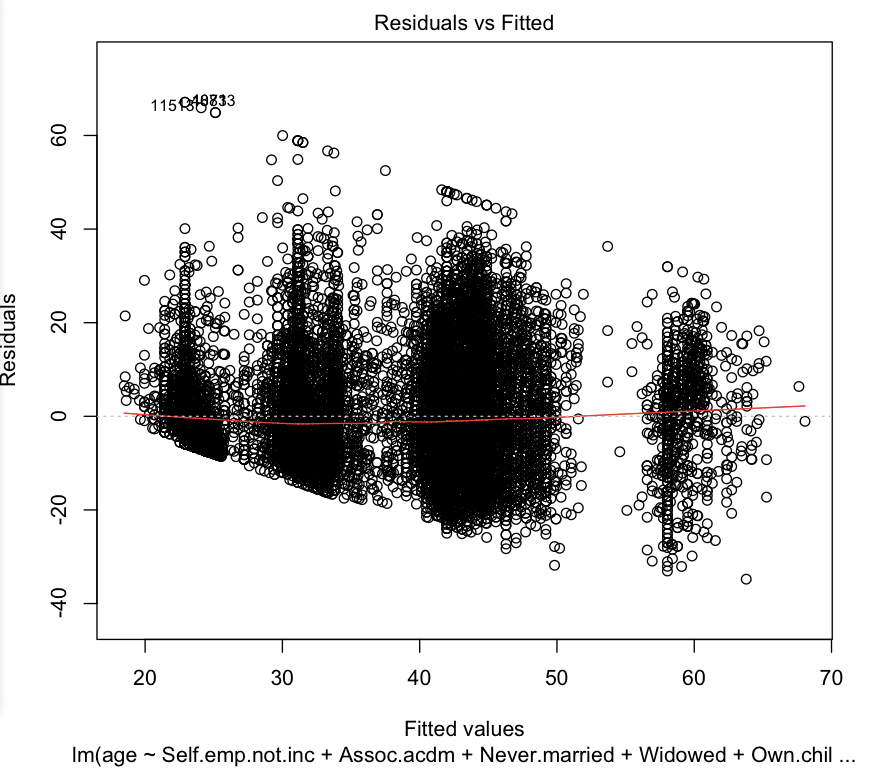
\includegraphics[scale=0.5]{figures/ageResidCensus.png}
 \caption{}
 \label{fig:ageResidCensus}
\end{figure}
 
 \begin{figure}
 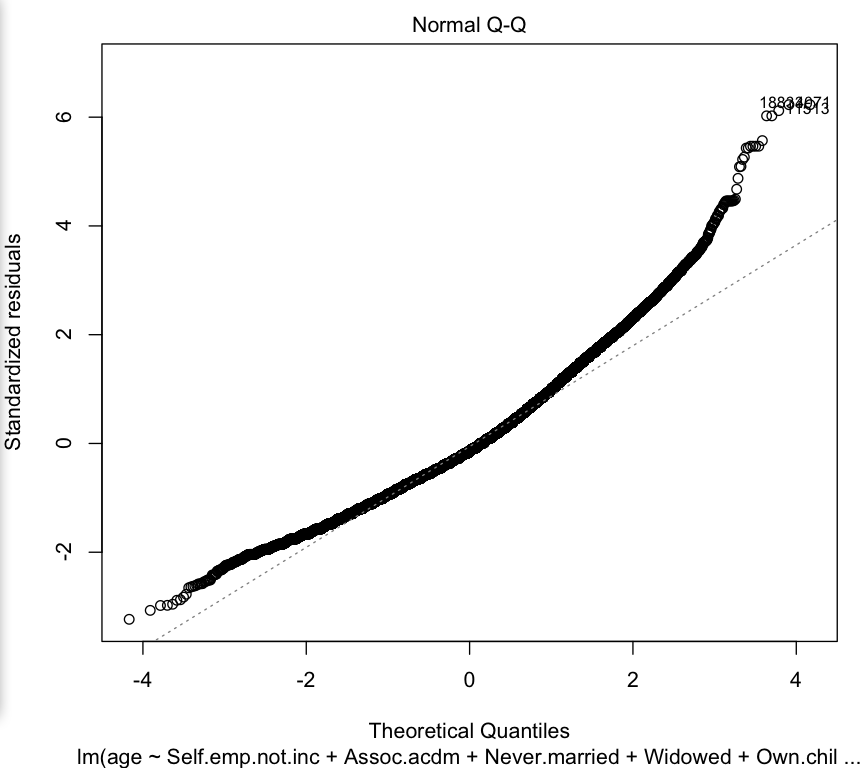
\includegraphics[scale=0.5]{figures/ageNormResidCensus.png}
 \caption{}
  \label{fig:ageNormResidCensus}
\end{figure}

\begin{figure}
 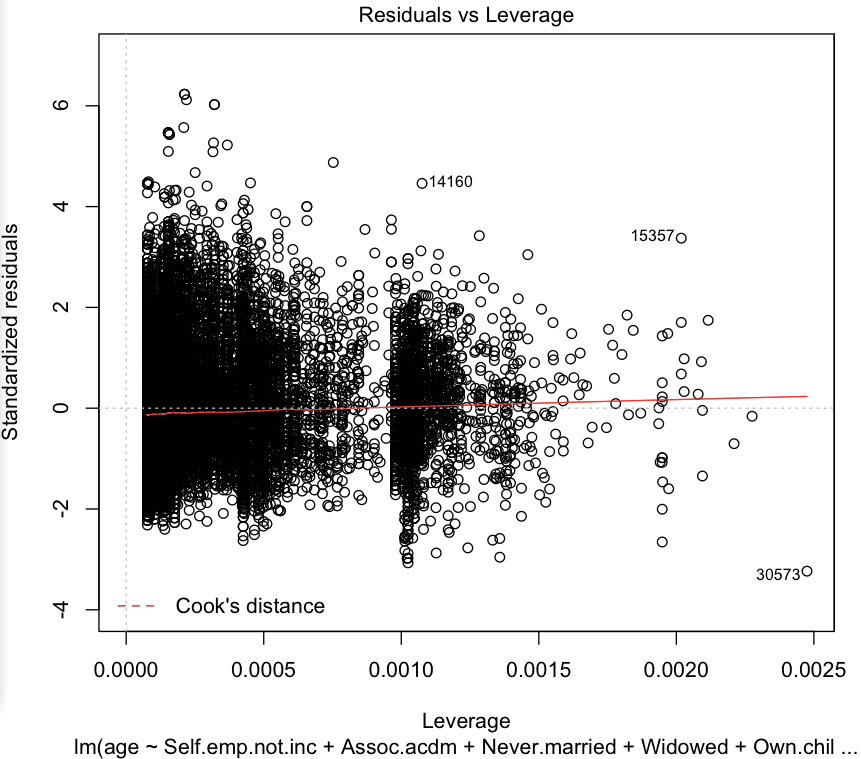
\includegraphics[scale=0.5]{figures/cookResidCensus.png}
 \caption{}
  \label{fig:cookResidCensus}
\end{figure}

Since many of the explanatory variables are categorical and age is not correlated in any straightforward way with the explanatory variables the model cannot be a perfect fit as seen in Figures~\ref{fig:ageResidCensus},~\ref{fig:ageNormResidCensus}. In fact there are many observations that have a very big impact on the model as Cook's distance plot shows (Figure~\ref{fig:cookResidCensus}).

\begin{figure}
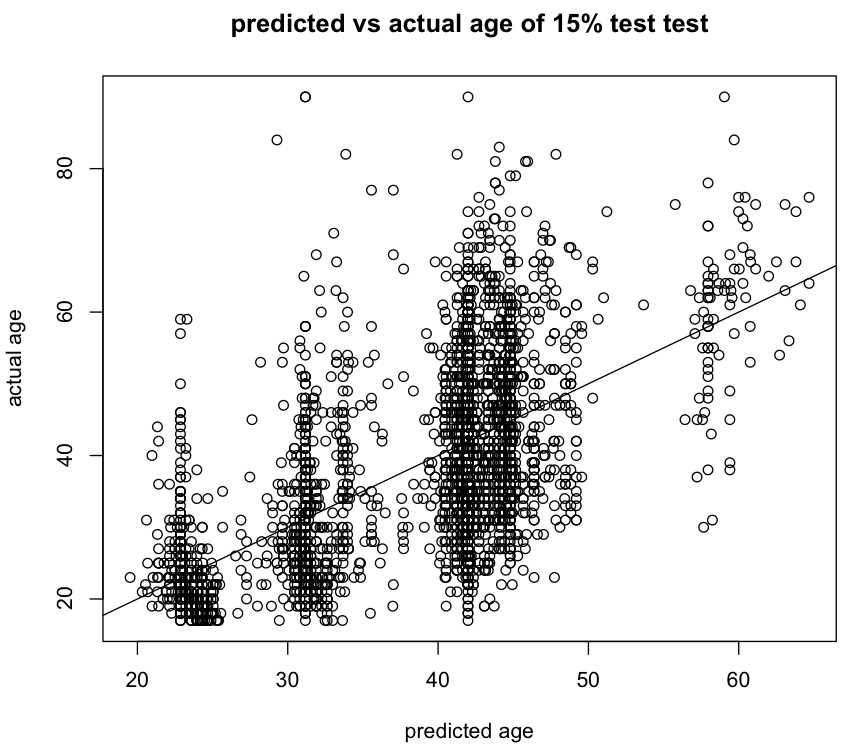
\includegraphics[scale=0.5]{figures/predVsActualCensus.png}
\caption{}
 \label{fig:predVsActualCensus}
\end{figure}

Since there are many more observations than we can visually assess, we decided to split the original data set in training(90\%) and test(10\%) subsets and to fit the train data but report the predicted versus actual values in the test data (Figure~\ref{fig:predVsActualCensus}). Now it is more clear that the age is clustered around 24, 32 and 40-45. The explanatory variables used aren't very good predictors for the person's age, unfortunately.

In order to consider the contribution of explanatory variables to the variance of age we sorted the 7 variables in order of their absolute correlation value with age. Then we adapted parsimony function to only work with this set and in the provided order so that we can produce and visualize the contribution of each variable in the most to least significance order as seen in Figure~\ref{fig:ageContrib}.

\begin{figure}
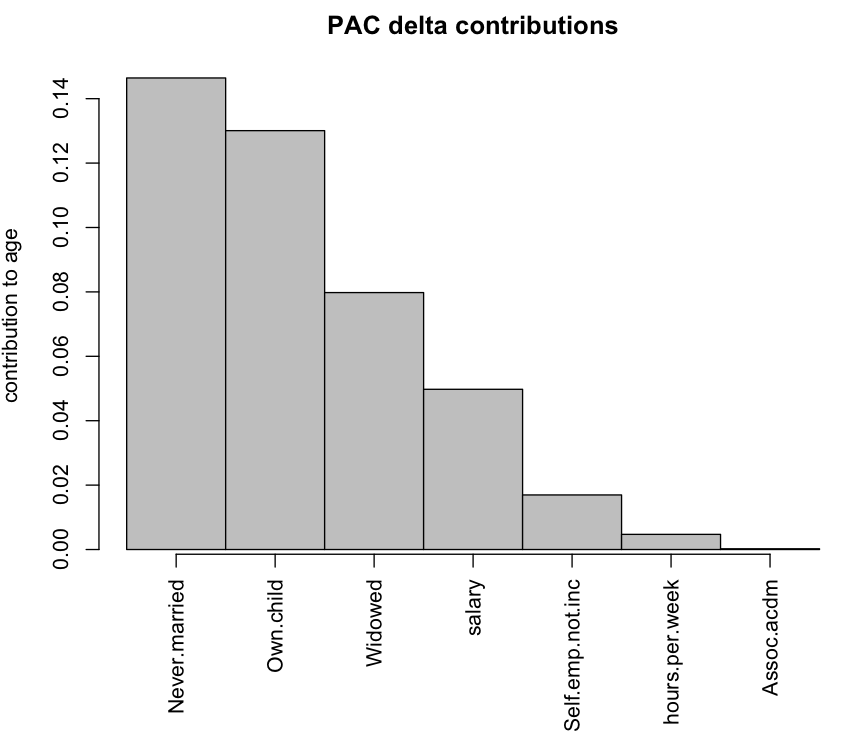
\includegraphics[scale=0.5]{figures/ageContrib.png}
\caption{}
 \label{fig:ageContrib}
\end{figure}

In all of the performed analyses the country of origin doesn't seem to play much of a role, or, perhaps, the country data is too sparse to be a good predictor of the outcome variables. Also it is interesting to point out that  education isn't highly correlated with the variables of interest when all of the explanatory variables are considered, since it didn't make it into the final models at k=0.01. It would be very interesting to compare these results with a more modern census information.

% Begin John Chen's Section

% Parsimony: Price Prediction (Linear)

% Table of Parsimonious Variables
For the small n (n \textless 1000), large p (p \textgreater 15) case, we will use the automobile data set found on the UCI Machine Learning Repository.

Here were the results of running prsm(): \\

\begin{center}
    \begin{tabular}{ | l |  p{4cm} |  p{4cm} | p{4cm} |}
    \hline
    Method & Parsimony (k = 0.01) & Parsimony (k = 0.05) & Significance Testing \\ \hline
    
    Columns Retained & ohcv, twelve-cylinders, engine.size, stroke, compression.ratio, peak.rpm & engine.size & bmw, dodge, `mercedes-benz`, mitsubishi, plymouth, porsche, saab, std, front, wheel.base, length, width, height, curb.weight, dohc, ohc, engine.size, peak.rpm\\ \hline
    
    AIC & 0.8676842 & 0.7888274 & 0.9308\\ \hline
    
    \end{tabular}
\end{center}

% Significance Testing Results
Summary of Significance Testing:\\
\begin{verbatim}
Coefficients:
              Estimate Std. Error t value Pr(>|t|)    
(Intercept) -5.360e+04  1.308e+04  -4.097 6.40e-05 ***
audi         1.628e+03  1.134e+03   1.436  0.15273    
bmw          8.537e+03  9.493e+02   8.992 4.02e-16 ***
dodge       -1.409e+03  9.491e+02  -1.484  0.13952    
mitsubishi  -2.507e+03  8.165e+02  -3.071  0.00248 ** 
plymouth    -1.390e+03  9.871e+02  -1.408  0.16096    
porsche      3.259e+03  2.497e+03   1.305  0.19345    
saab         2.994e+03  1.154e+03   2.593  0.01031 *  
std         -1.303e+03  5.721e+02  -2.277  0.02399 *  
front       -1.292e+04  2.976e+03  -4.343 2.38e-05 ***
wheel.base   1.644e+02  8.338e+01   1.972  0.05022 .  
length      -1.543e+02  4.576e+01  -3.372  0.00092 ***
width        9.632e+02  2.354e+02   4.092 6.55e-05 ***
height      -1.879e+01  1.279e+02  -0.147  0.88334    
curb.weight  3.625e+00  1.246e+00   2.909  0.00411 ** 
dohc         1.512e+03  8.983e+02   1.683  0.09422 .  
ohc          1.082e+03  5.095e+02   2.124  0.03511 *  
engine.size  9.950e+01  1.111e+01   8.954 5.10e-16 ***
peak.rpm     1.107e+00  4.399e-01   2.517  0.01274 *  
\end{verbatim}

\newpage

% Parsimony: Is this car relatively safe? (Logistic)

For the logistic regression case, we seek to find most effective variable, when it comes to determining how safe a car is.  In the original data set, each car is assigned a safety rating ranging from -3 to 3.  This range of values was converted into a discreet indicator variable - 1 if the car is relatively safe, having scored 1 or higher on the original scale.

% Table of Parsimonious Variables

Here are the results of running prsm():\\
\begin{center}
    \begin{tabular}{ | l |  p{4cm} |  p{4cm} | p{4cm} |}
    \hline
    Method & Parsimony (k = 0.01) & Parsimony (k = 0.05) & Significance Testing \\ \hline
    	
    Columns Retained & saab, toyota, volkswagen, turbo, two-doors, hatchback, sedan, 4wd, rwd, rear, wheel.base, length, width, height, curb.weight, l, ohc, ohcf ,ohcv, five-cylinders, four-cylinders, three-cylinders, twelve-cylinders, engine.size, 2bbl, idi, mfi, mpfi, spdi, bore, stroke, compression.ratio, horsepower, peak.rpm, city.mpg, highway.mpg & saab, toyota, volkswagen, turbo, two-doors, hatchback, sedan, 4wd, rwd, rear, wheel.base, length, width, height, curb.weight, l, ohc, ohcf ,ohcv, five-cylinders, four-cylinders, three-cylinders, twelve-cylinders, engine.size, 2bbl, idi, mfi, mpfi, spdi, bore, stroke, compression.ratio, horsepower, peak.rpm, city.mpg, highway.mpg & audi, saab, volkswagen, diesel, std, four-doors, 4wd, fwd, 1bbl\\ \hline
    
    AIC & 74 & 74 & 56\\ \hline
    
    \end{tabular}
\end{center}


% Significance Testing

\texttt{Summary of Significance Testing:}\\
\begin{verbatim}
Coefficients:
              Estimate Std. Error t value Pr(>|t|)    
(Intercept)   0.806479   0.074888  10.769  < 2e-16 ***
audi          0.590168   0.140289   4.207 4.05e-05 ***
saab          0.323690   0.140778   2.299 0.022618 *  
volkswagen    0.241768   0.105225   2.298 0.022715 *  
diesel       -0.165675   0.093946  -1.764 0.079483 .  
std          -0.002151   0.069947  -0.031 0.975495    
`four-doors` -0.674964   0.049956 -13.511  < 2e-16 ***
`4wd`        -0.038044   0.126373  -0.301 0.763724    
fwd           0.208747   0.054731   3.814 0.000187 ***
`1bbl`       -0.313088   0.106989  -2.926 0.003864 ** 

\end{verbatim}
 %End John Chen's Section
 
%%%%%%%%%%%%%%%%%%

\section*{Problem 2.d}

See \texttt{Leave.R} for the code.

Our results are below. The only potentially interesting difference is that this PAC discards one additional variable, Genetics or Pedigree. (depending on where the label came from) This was the biggest loss the Leave-One-Out PAC took, but it still cost less than a percent of accuracy. Perhaps it was just outside of the  k-value range for \textbf{aiclogit} to throw it out, or this PAC is slightly compressed compared to \textbf{aiclogit}.

\begin{verbatim}
> leaveTest()
full outcome =  0.7682292 
deleted         blood_pressure 
new outcome  =  0.7669271 
deleted         skin_thickness 
new outcome  =  0.7669271 
deleted         insulin 
new outcome  =  0.7695312 
deleted         pedigree 
new outcome  =  0.7630208 
deleted         age 
new outcome  =  0.7630208 
[1] "pregnancies"     "plasma"          "body_mass_index"
\end{verbatim}




%%%%%%%%%%%%%%%%%%


\begin{thebibliography}{99}
    
     \bibitem{pima} Instances of diabetes in the Pima Indians. $p=9, n=769$ Stored locally in \textbf{pima.csv}. Downloaded from \url{https://archive.ics.uci.edu/ml/machine-learning-databases/pima-indians-diabetes/} 
  
    \bibitem{census} Adult Data Set, compiled from Census of 1994. $p=14 \rightarrow 110$ after factor variables expanded into their own 0-1 vectors, $n=32561$ Stored locally in \textbf{census.csv}. Downloaded from \url{https://archive.ics.uci.edu/ml/datasets/Adult} 
    
    \bibitem{cadata} California Housing Data.  $p = 8, n=20640$. Stored locally in \textbf{cadata.csv}. Downloaded from \url{http://lib.stat.cmu.edu/datasets/houses.zip}
	
	\bibitem{shuttle} Shuttle Data.  $p = 9, n = 58000 \rightarrow 43500$ for training, $14500$ for testing. Stored locally in \textbf{shuttle\_training.csv} and \textbf{shuttle\_testing.csv}. Downloaded from \url{https://archive.ics.uci.edu/ml/datasets/Statlog+\%28Shuttle\%29}
    
    \bibitem{abalone} Abalone Data Set. $p = 8, n = 4177$. Stored locally in \textbf{abalone.csv}. Nominal Sex variable changed from F,M,I (Male, Female or Infant) into is.male and is.infant (each 0-1 valued). Downloaded from \url{https://archive.ics.uci.edu/ml/datasets/Abalone}
    
    \bibitem{automobile} Automobile Data Set. $p = 26 \rightarrow 70$ after factor variables expanded into their own 0-1 vectors, $n = 205 \rightarrow 194$ after NA removal. Stored locally in \textbf{imports-85.csv}. Downloaded from \url{https://archive.ics.uci.edu/ml/datasets/Automobile}
    
\end{thebibliography} 
 
\end{document}
